\chapter{21\ cm Interferometry}
\label{ch2}

To overcome the challenges associated with foreground removal, and to acquire enough observing time
to detect the faint hydrogen signal, we primarily use instruments that are either
dedicated to 21\ cm cosmology or designed with it as a primary goal.  This section will describe
the principles of the instruments and the specific ones used by our group.

\section{Interferometry}

21\ cm cosmology experiments are primarily (but not exclusively) a type of radio telescope called an
\emph{interferometer}.  Interferometers (as opposed to ``single dish" radio telescopes) consist of a
large number of antennas which are connected to a central (super-)computer called a \emph{correlator}.
The job of the correlator is to take the signal from every antenna and correlate it with the 
signal from every other antenna.  So, for example, an array with 128 independent antennas will
produce 8,128 independent correlations.  

A principal advantage of interferometers is that they can make high resolution images over a large
area of the sky.  For a single dish telescope, both the resolution and the field of view
(i.e. how much of the sky the telescope is sensitive to at any given time) are the same --- i.e.
a single dish telescope can be thought of as a single pixel camera.  To make images, a single dish
scans its one pixel across the sky.  For an interferometer, however, 
the resolution is effectively set by the largest antenna separation, while the field of view is
set by the size of any single antenna in the array.  So for example, an interferometer 300 meters
across, with individual antenna elements 10 meters in size, has the same resolution as a 300 meter
single dish telescope --- but a field of view 900 times bigger!

The process of actually making images from interferometers, however, is fairly complicated.  In my
experience, interferometry is a skill best learned hands-on.  The basic principle (which I will not
attempt to explain here) is that each
pair of antennas (called a ``baseline") measures only a single Fourier mode of the sky.  To reconstruct
an image of the sky, one needs to measure a large number of different Fourier modes (i.e. have a lot of
different baselines).  Then one can simply perform an inverse Fourier transform and get an image.
In practice, things are never so simple, but that's where all the fun lies.

Resources for learning more about interferometry are, unfortunately, somewhat spotty. 
\cite{fomalont_and_wright_1974} is probably my favorite from a pedagogical perspective, 
but it predates modern computers, and so some of its content is hopelessly out of date.  (The actual
article is hard to find --- if you are interested in reading it, I can get you a copy.)
The National Radio Astronomy Observatory hosts a bi-annual summer school on interferometry,
which published its lectures in a textbook that is freely available \citep{taylor_et_al_1999}.
It is also rather out of date, although a new version is rumored.
The ultimate, comprehensive resource is a textbook called ``Interferometry and Synthesis in
Radio Astronomy" \citep{thompson_et_al_2001}.  It contains everything you'd ever want to know
and much, much more.  Unfortunately, it's hard to skim or to find information on specific topics only,
and so it not too useful as an introductory resource.

\section{Interferometric Data}

While working with real data and real telescopes is probably the best way to get familiar
with the concepts of interferometry, it's worthwhile to say a few words about what data from
interferometers look like.  The first thing to note is that interferometric data ---
called ``visibilities" --- consists of complex numbers.  This is because a correlator
returns a measurement in Fourier space, and even if the sky is real-valued (which it is),
the Fourier transform of the sky is complex.  Complex numbers consist of a real part
and an imaginary part, but for interferometry it is much more useful to think of them
in polar coordinates on the complex plane: as an amplitude and a phase.  In general,
amplitudes of visibilities tell you how bright sources on the sky are, whereas the phase
tells you where those sources are located.

The second thing to mention is that there are two principal types of correlations:
auto-correlations, in which the measurements from an antenna are correlated with themselves,
and cross-correlations, in which the measurements from an antenna are correlated with
those from another antenna (i.e. the measurements are from one baseline).
Cross-correlations contain nearly all the astrophysically
relevant data.  An auto-correlation is basically a single dish antenna, which as stated above,
has very limited resolution if the dish is small.  As such, cross-correlations form the key
components of our measurements.  However, auto-correlations can be very useful for diagnosing
any problems with a system, as they measure the total power received by the antenna (with
no information about the distribution of that power on the sky).  Note that auto-correlations
are purely real-valued, i.e., they have a phase of zero.

The last thing to mention is that interferometers make measurements as a function of frequency
and time.
A typical (modern) instrument can have 1,000 different frequency channels over its measurement
bandwidth.  The time resolution of an instrument can vary, but typically visibilities
are integrated to a timescale of several seconds.  As such, the most useful way to visualize 
interferometric data is in a ``waterfall" plot, as shown in Figure \ref{fig:waterfall}.
A waterfall plot has time on one-axis (typically $y$, although one shouldn't assume),
and frequency on the other.  It can plot either the amplitude or phase (Figure
\ref{fig:waterfall} shows the amplitude on a logarithmic color scale) from one baseline.
\begin{figure}[htbp!]
\centering
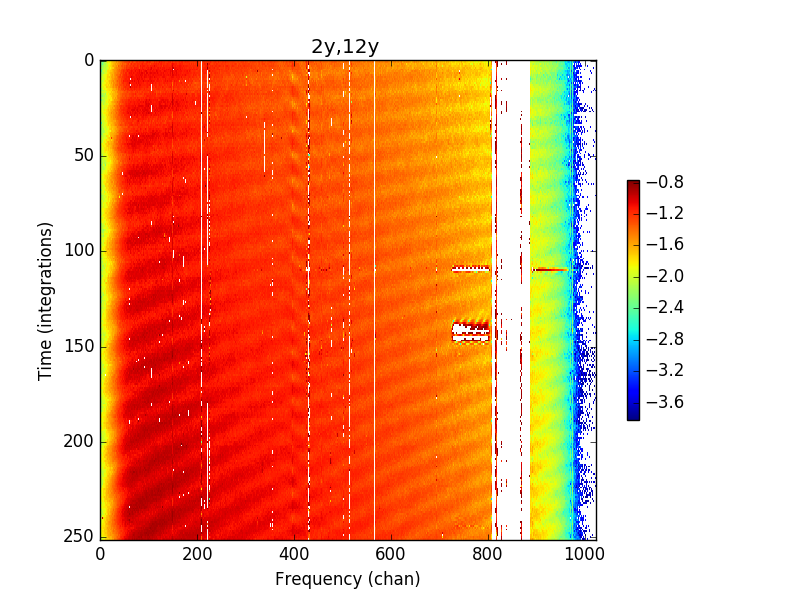
\includegraphics[width=4.5in]{figures/waterfall.png}
\caption{A waterfall plot of the amplitude (on a logarithmic color scale) from one baseline.  White
areas correspond to data that has been identified as contaminated by radio frequency interference
and removed.}
\label{fig:waterfall}
\end{figure}


\section{The Instruments}

Our group primarily uses data from three instruments: the Precision Array for Probing the
Epoch of Reionization (PAPER), the Murchison Widefield Array (MWA), and the
Hydrogen Epoch of Reionization Array (HERA).

\subsection{PAPER}

PAPER was an interferometer consisting of 128 antennas in the Karoo desert of South Africa.
(All of these experiments are located in isolated ``radio quiet" zones to avoid interference.)
\begin{figure}[ht]
\centering
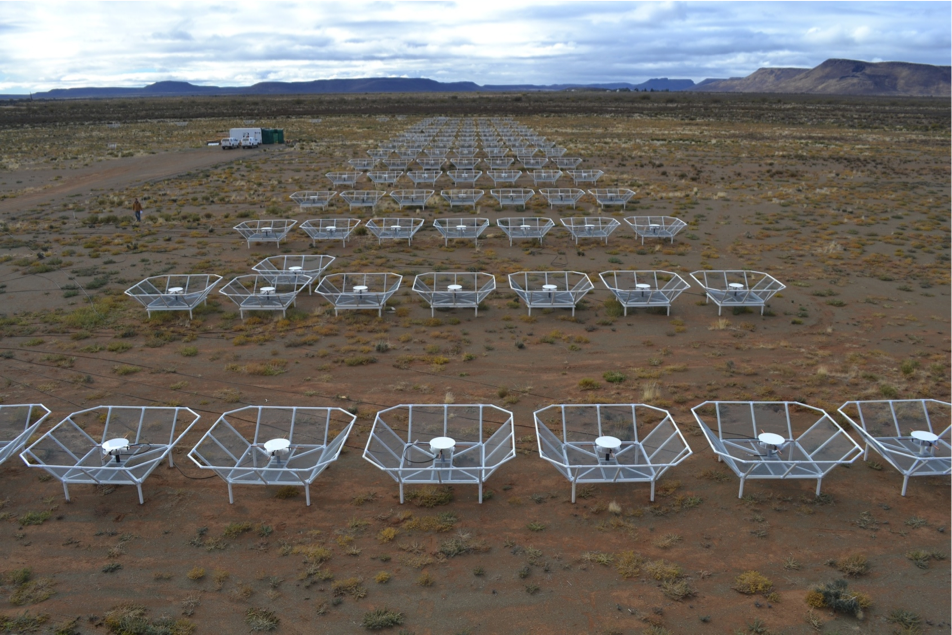
\includegraphics[width=4.5in]{figures/paper.png}
\caption{The final array configuration for the PAPER 128 experiment in South Africa.}
\label{fig:paper}
\end{figure}
An image of the final PAPER layout is shown in Figure \ref{fig:paper}.
You may notice that PAPER seems to fly in the face of everything I told you about interferometry
above.  Rather than consisting of many different baselines, PAPER has a large amount of 
redundancy, i.e., pairs of antennas that measure the exact same Fourier mode on the sky.
PAPER also is not very large, with its longest baseline only $\sim 300$ meters, which gives
it poor resolution.  The key principle behind PAPER lies in the fact that first generation
21\ cm cosmology experiments are \emph{not} trying to image the structure of reionization.
Rather, to make a statistical detection using the power spectrum, a redundant configuration
like PAPER can provide a significant sensitivity boost while also enabling a unique set of
analysis tools.  PAPER was, in effect, de-commissioned in 2015 to build HERA, although many
PAPER antennas are still operational and the final analysis of PAPER data is still ongoing.


\subsection{MWA}

The MWA is an interferometer consisting of 256 antennas located in the Western Australian
outback. An MWA ``antenna" actually consists of 16 different antennas comprising a single ``tile".
This design choice effectively narrows the field-of-view of the MWA while increasing
sensitivity.  Three MWA tiles are shown in Figure \ref{fig:mwa}.
\begin{figure}[htbp!]
\centering
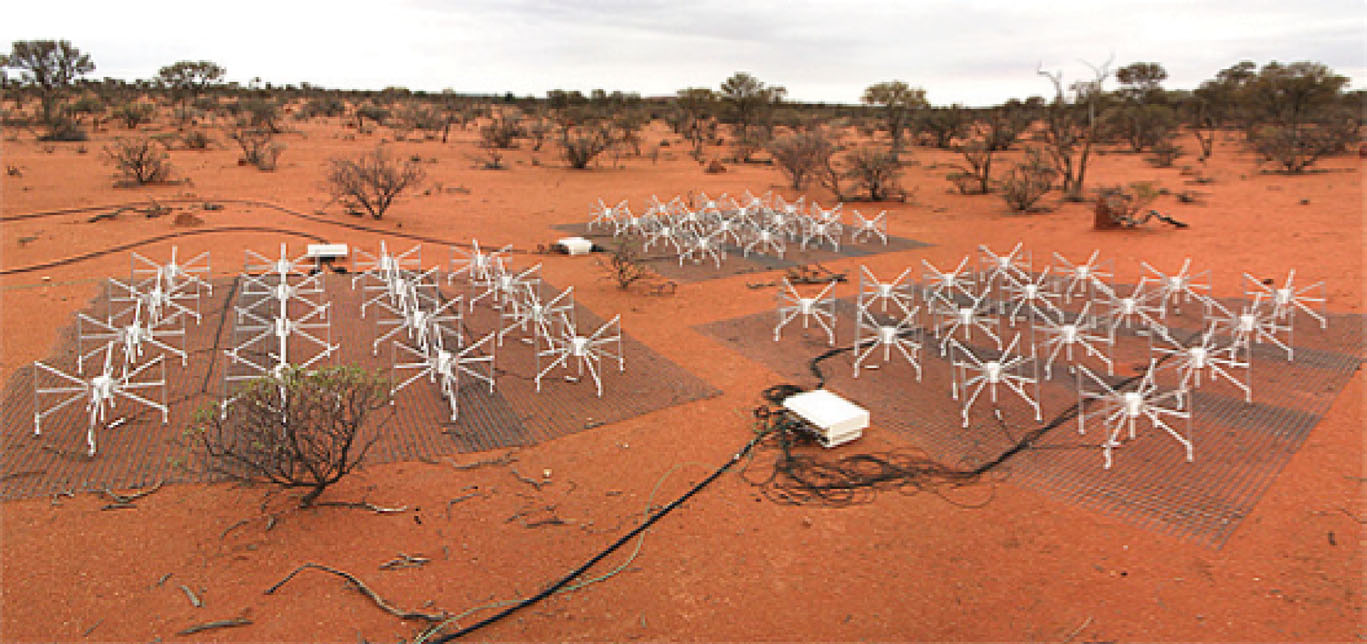
\includegraphics[width=4.5in]{figures/mwatile.jpg}
\caption{Three tiles of the MWA, each consisting of 16 antenna which are connected to a combiner
called a ``beamformer" before the signals are sent to the correlator.}
\label{fig:mwa}
\end{figure}
The MWA tiles are spread in a semi-random configuration, with a high number of tiles concentrated
near the center, but the longest baselines stretch out to 5 kilometers.  This gives
the MWA good sensitivity to the 21\ cm EoR signal while also making it a good imager.
In this case, however, the goal is not to image the EoR but to image the foregrounds so they can be
modeled and removed, enabling a detection of the EoR power spectrum.
Note that a 128 tile version of the MWA, now referred to as Phase I, completed
observations in 2016.  Phase II, currently underway, consists of 256 tiles but can only correlate
128 of them at a time.  It operates in an EoR mode, where the 128 tiles are concentrated near 
the center, including two sets of redundantly spaced tiles to enable analysis in the PAPER style,
and a long-baseline mode, where the tiles are spread very far apart to give high resolution.  
Plans for a Phase III MWA that can correlate all 256 tiles are underway.

\subsection{HERA}

HERA is the newest 21\ cm cosmology experiment and is still under construction.  An
image of HERA taken in 2016 can be seen in Figure
\ref{fig:hera}, while a rendition of the full array is shown in Figure \ref{fig:hera_render}.
\begin{figure}[htbp!]
\centering
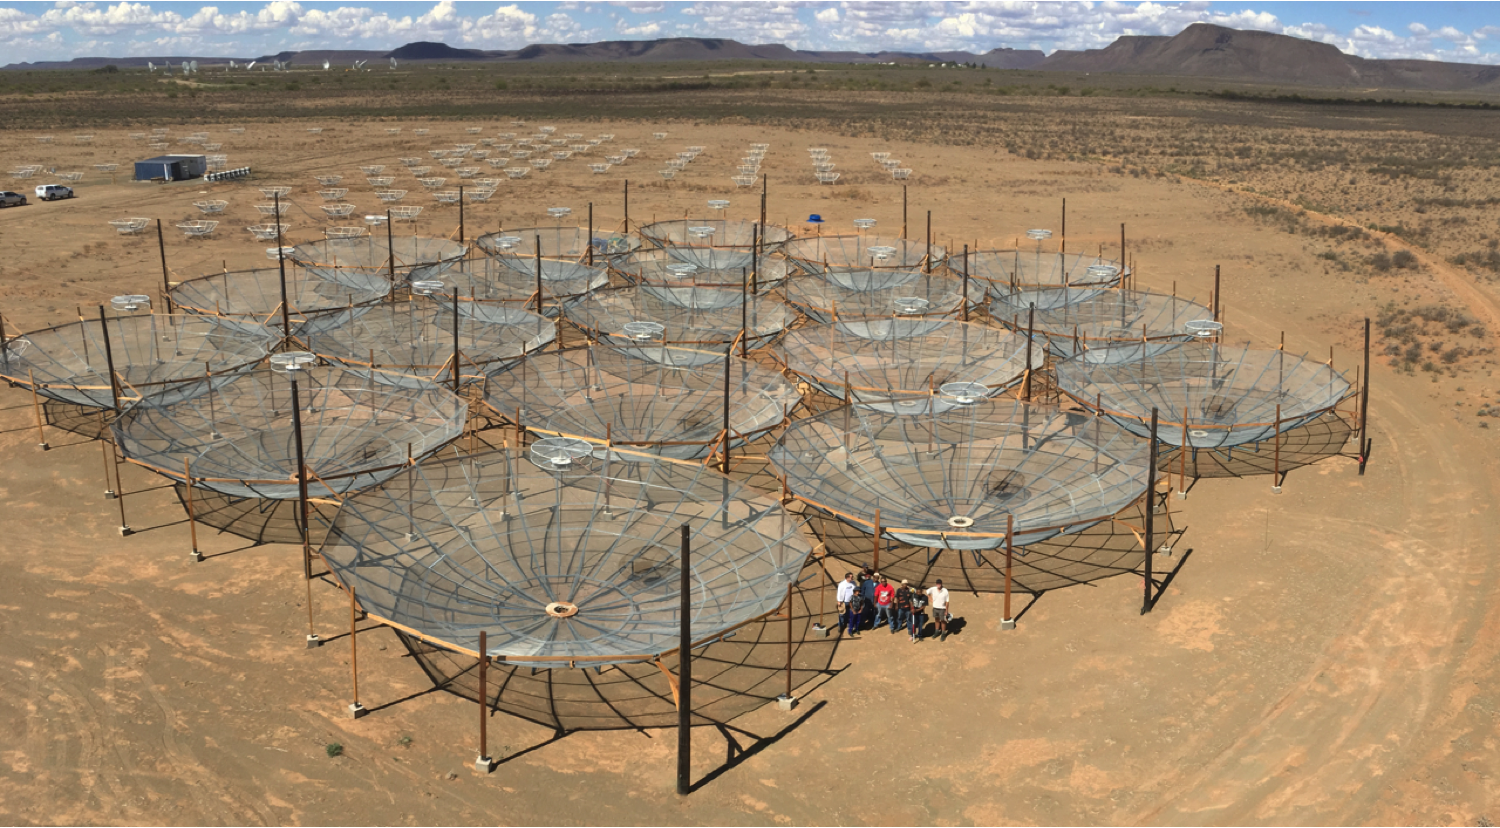
\includegraphics[width=4.5in]{figures/HERA.png}
\caption{The 19 dishes in the prototype HERA array.}
\label{fig:hera}
\end{figure}
\begin{figure}[htbp!]
\centering
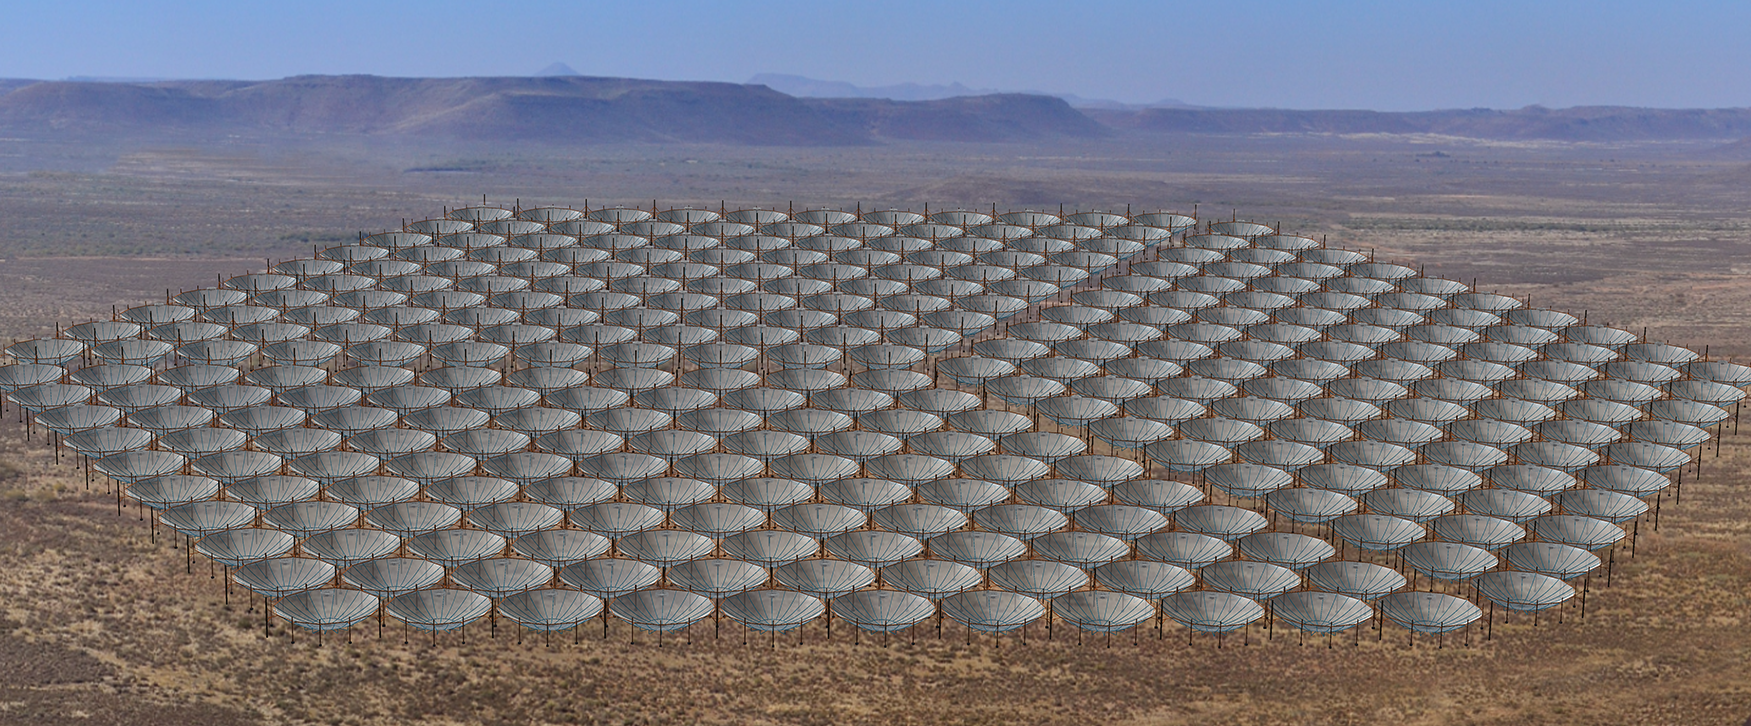
\includegraphics[width=4.5in]{figures/hera_render.png}
\caption{A rendition of the core of the full 350 dish HERA.  The core will be over 300 meters
across.}
\label{fig:hera_render}
\end{figure}
HERA is located on the former PAPER site in South Africa (a number of PAPER antennas can be
seen in the background of Figure \ref{fig:hera}) and uses much of the same infrastructure as
PAPER.  The biggest change is the switch to large dish antennas, each of which spans 14 meters.  This
increase in size will give HERA significantly more sensitivity than any existing 21\ cm EoR
experiment.  HERA combines knowledge from both the MWA and PAPER, and the layout reflects this:
it has a large number of redundant baselines, but enough different types to function as a high
fidelity imager. 
